% !TEX encoding = UTF-8
% !TEX TS-program = pdflatex
% !TEX root = ../tesi.tex

%**************************************************************
\chapter{Analisi dei requisiti}
\label{cap:analisi-requisiti}
%**************************************************************
\intro{In questo capitolo viene descrive la fase di analisi dei requisiti effettuata per
la realizzazione del progetto.}

\section{Scopo del progetto}
Uno sviluppatore prima di me ha realizzato un set di REST API per gestire le funzionalità del progetto Smart Parking 
e un servizio di polling che va a prendere lo stato dei sensori di parcheggio, aggiornato 
in un file XML online e salva le variazioni nel servizio di persistenza.
\\\\
Lo scopo di questo progetto è migrare le REST API e il servizio di polling, dalla soluzione
realizzata con il framework Spring, in una soluzione realizzata con il framework NestJS.

\section{Confronto con gli stakeholders}
E' stato fatto un incontro iniziale con il proponente, ovvero l'azienda Sync Lab,
per definire con chiarezza i requisiti richiesti.
\subsection{Servizio REST API}
Nell'incontro sono state prese in considerazione le REST API esistenti (realizzate con il framework Spring) 
di cui doveva essere fatta la migrazione.
E' emerso subito che la quantità di REST API da realizzare era troppo elevata per il
tempo di stage a disposizione. 
\\\\
E' stato quindi necessario fare una valutazione di quali fossero i servizi fondamentali che
il servizio di REST API avrebbe dovuto esporre, per poter essere utilizzato senza che venissero
a mancare funzionalità fondamentali per un utilizzo a livello base del sistema.

\subsection{Servizio di polling}
Abbiamo poi valutato il secondo punto importante per questo progetto, ovvero
la necessità di avere le informazioni sullo stato dei sensori sempre aggiornate.
\\\\
La rete dei sensori cresce in maniera dinamica, in quanto un nuovo sensore viene aggiunto/spostato
da un parcheggio senza che un utenza manuale informi il sistema. 
\\
Ma è necessario che quando un sensore si aggiunge alla rete, il sistema lo rilevi e ne mantenga lo stato
aggiornato. La stessa cosa deve avvenire per quanto riguarda lo spostamento di un sensore, solo che in 
questo caso il sistema deve aggiornare le coordinate del sensore esistente, anziché aggiungerne uno nuovo.
\\\\
Sono stati scelti una tipologia di sensori con GPS integrato, che ad ogni variazione di stato vanno ad 
aggiornare un record a loro associato in un file XML online, dove ogni record contiene le informazioni e
lo stato del sensore.
% //TODO: inserie immagine file XML sensori
\\\\
Non avendo controllo sui sensori e quindi su dove vengano scritti i dati, con la proponente si è deciso
di effettuare un polling ogni due minuti al file XML e aggiornare lo stato del back-end.
\\\\
Lo stato dei sensori è quindi ridondante in quanto è presente sia nel back-end del progetto che sul file XML online. 
La scelta di duplicare lo stato dei sensori nel back-end è stata fatta per trarne i seguenti benefici:
\begin{itemize}
    \item permette di organizzare i dati in maniera più consona e organizzata.
    \item l'accesso ai dati diventa molto più veloce in quanto non si deve interrogare un file XML online
        in una posizione remota e sconosciuta ma viene interrogato il servizio di persistenza del back-end, 
        di cui abbiamo pieno controllo.
\end{itemize}
\leavevmode\newline
La motivazione che ha portato ad eseguire il polling ogni due minuti è la seguente:
\\
il tipo di servizio offerto non ha bisogno di essere un real-time system, in quanto non crea problemi all'utente
vedere una piazzola che si libera/occupa con un delta di intervallo di ritardo. 
\\\\
L'importante è che questo delta non sia troppo elevato, in tal caso i dati mostrati agli utenti sarebbero troppo
inconsistenti per risultare utili. Mentre un delta troppo piccolo genera un carico di lavoro per l'applicazione molto
elevato.
\\\\
Infatti effettuare il polling con un piccolo intervallo di tempo tra un polling e il successivo (dell'ordine dei millisecondi
ad esempio),
genera la produzione di molte 
chiamate http da parte del back-end per accedere al contenuto del file XML e molti accessi al database in caso ci siano dati da 
inserire/aggiornare.
\\\\
Vediamo un esempio pratico con una tabella che mostra il costo di chiamate e accessi al database giornalieri al variare 
dell'intervallo di tempo del polling:
\\
% //TODO: aumentare altezza celle tabelle
% //TODO: aggiungere caption immagini
% //TODO: ridimensionare immagini
\begin{table}
    \begin{tabular}{|p{2.85cm}|p{3.05cm}|p{3.05cm}|p{3.35cm}|} 
    \hline
    \textbf{Polling} & \textbf{\# chiamate http}  & \textbf{\# accessi lettura} & \textbf{\# accessi scrittura} \\ 
    \hline
    60 minuti & 24 & 24 * $10^3$ & 24 * $10^3$ \\
    \hline
    30 minuti & 48 & 48 * $10^3$ & 48 * $10^3$ \\
    \hline
    15 minuti & 96 & 96 * $10^3$ & 96 * $10^3$ \\
    \hline
    5 minuti & 288 & 288 * $10^3$ & 1440 * $10^2$ \\
    \hline
    2 minuti & 720 & 720 * $10^3$ & 1440 * $10^2$ \\
    \hline
    1 minuto & 1440 & 1440 * $10^3$ & 1440 * $10^2$ \\
    \hline
    1 millisecondo & 864 * $10^5$ & 864 * $10^8$ & 1440 * $10^2$ \\
    \hline
    \end{tabular}
\end{table}
\leavevmode\newline
\\
Per calcolare il numero medio di accessi al database è stata ipotizzata la presenza di 1000 sensori a sistema e che 
ogni cinque minuti la metà dei sensori abbiano bisogno di un aggiornamento (quindi 100 sensori devono essere 
acceduti in scrittura ad ogni minuto). 
\\\\
Quindi si verificano 1000 accessi in lettura ad ogni polling per verificare quali abbiano bisogno di aggiornamento.
Gli accessi in scrittura variano in base al tempo trascorso dall'ultimo polling (da ricordare che gli accessi in scrittura sono molto
più costosi di quelli in lettura).
\\\\
Come vediamo dalla tabella e come auspicabile, con il polling ad un intervallo di ogni ora si effettuano solo
24 richieste http al giorno ma il delta di latenza di aggiornamento dei dati ad ogni ora li rende inutilizzabili.
\\\\
D'altra parte un intervallo di un millisecondo rende i dati aggiornati quasi in tempo reale ma 
non è sostenibile effettuare un numero di richieste giornaliere dal back-end pari a 864 * $10^5$ (più di 86 milioni).
\leavevmode
\\\\
Un numero di richieste giornaliere pari a 720 è stato ritenuto accettabile, così come il numero di accessi al database
indicati per la colonna dei 2 minuti e si è optato quindi per questa scelta; ritenendo il delta di ritardo di
aggiornamento un valore accettabile per l'utente finale e che i costi delle chiamate e di accessi al database non
siano di sovraccarico per il sistema.
\\\\
Il servizio per il polling dei sensori deve essere realizzato in modo che sia separato da quello delle REST API.
\\
Sia per una separazione di responsabilità, che per una futura migrazione a un'applicazione basata su microservizi,
in cui il servizio di polling deve diventare un microservizio a se stante, gestibile in maniera indipendente rispetto
agli altri microservizi.

\section{Entità}
Per rendere più chiaro il dominio del progetto ed eliminare eventuali ambiguità, si è ritenuto necessario
documentare le entità di dominio coinvolte nelle funzionalità fondamentali delle REST API.
\\\\\\
\textbf{Piazzola}
\\\\
Modella il rettangolo bianco dipinto sull'asfalto che delimita la zona in cui l'automobile viene messa
in sosta. Ogni piazzola deve essere associata ad un parcheggio. Una piazzola può avere un solo sensore
di parcheggio.
\\
Ogni piazzola è caratterizzata da:
\begin{itemize}
    \item id: numero incrementale.
    \item latitudine: stringa.
    \item longitudine: stringa.
\end{itemize}
\leavevmode\newline
\textbf{Parcheggio}
\\\\
Modella l'insieme di piazzole.
\\
Ogni parcheggio è caratterizzato da:
\begin{itemize}
    \item id: numero incrementale.
    \item latitudine: stringa.
    \item longitudine: stringa.
\end{itemize}
\leavevmode\newline
\textbf{Sensore}
\\\\
Modella il sensore. Esistono due tipi di sensore:
\begin{itemize}
    \item ambientale: misurana la qualità dell'aria e altri parametri nel parcheggio e possono 
        coprire un'area di N piazzole.
        Sono gestiti da un'altro progetto di tirocinio, quindi non sono facenti parte di questo dominio di progetto.
    \item di parcheggio: sensore posizionato sotto l'auto nella piazzola. Rileva la presenza o meno
        del veicolo. Questo tipo di sensore può essere associato a una sola piazzola.
\end{itemize}
Ogni sensore può avere una sola azienda manutentrice a lui associata.
Ogni sensore è caratterizzato da:
\begin{itemize}
    \item id: numero incrementale.
    \item nome: stringa.
    \item batteria: stringa, indica la tensione della batteria in Volt.
    \item carica: stringa, indica il livello di carica della batteria (da 1 a 3).
    \item type: stringa, indica il tipo di sensore (ambientale o di parcheggio).
    \item attivo: booleano.
    \item ultimo sondaggio: timestamp, indica l'ultima volta che è stato aggiornato lo stato del sensore.
    \item da riparare: booleano, indica se il sensore deve essere riparato.
    \item da caricare: booleano, indica se la batteria del sensore è scarica.
    \item in aggiornamento: booleano, indica se il sensore sta aggiornando il suo software.
\end{itemize}
\leavevmode\newline
\textbf{Manutentore}
\\\\
Modella l'azienda incaricata alla manutenzione dei sensori.
Ogni manutentore è caratterizzato da:
\begin{itemize}
    \item id: numero incrementale.
    \item nome: stringa, indica il nome del titolare dell'azienda.
    \item cognome: stringa, indica il cognome del titolare dell'azienda.
    \item azienda: stringa.
    \item telefono: stringa.
    \item email: stringa.
\end{itemize}
\leavevmode\newline
\textbf{Misurazione sensore parcheggio}
\\\\
Modella la misurazione effettuata dal sensore di parcheggio. A differenza di un sensore ambientale, un sensore
di parcheggio non salva uno storico di misurazioni fatte ma viene inserita solo l'ultima misurazione effettuata,
sovrascrivendo la precedente.
Ogni misurazione di un sensore di parcheggio è caratterizzata da:
\begin{itemize}
    \item id: numero incrementale.
    \item indirizzo: stringa.
    \item latitudine: stringa.
    \item longitudine: stringa.
    \item valore: booleano, indica se il veicolo è presente o meno sopra al sensore.
    \item marca temporale: timestamp, indica la data in cui è stata effettuata la misurazione.
\end{itemize}

\section{Casi d'uso}
Definite le entità di dominio si è proceduto con la creazione dei casi d'uso.
\\
Per maggior chiarezza i casi d'uso sono stati raggruppati per entità di dominio di appartenenza.
\\\\
% parcheggio
\begin{figure}[!h]
    \centering
    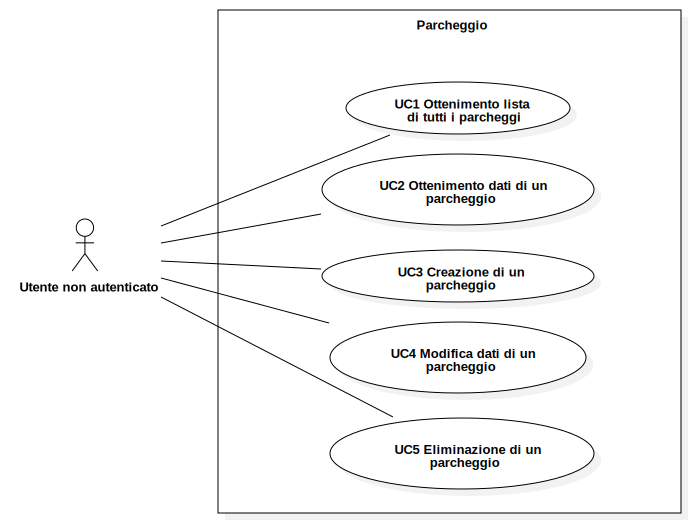
\includegraphics[height=9cm]{usecase/parking-area}
\end{figure}
\leavevmode\newline
\textbf{UC1 - Ottenimento lista di tutti i parcheggi}
\\\\
\textbf{Attori primari:} utente non autenticato.
\\
\textbf{Precondizioni:} l'utente è in possesso degli strumenti per poter effettuare la richiesta al sistema.
\\
\textbf{Post-condizioni:} l'utente ha ottenuto una lista di tutti i parcheggi.
\\
\textbf{Scenario principale:}
\begin{enumerate}
    \item l'utente richiede la lista di tutti i parcheggi.
    \item l'utente ottiene una lista di tutti i parcheggi.
\end{enumerate}
\leavevmode\newline
\textbf{UC2 - Ottenimento dati di un parcheggio}
\\\\
\textbf{Attori primari:} utente non autenticato.
\\
\textbf{Precondizioni:} l'utente è in possesso degli strumenti per poter effettuare la richiesta al sistema.
\\
\textbf{Post-condizioni:} l'utente ha ottenuto i dati di un parcheggio.
\\
\textbf{Scenario principale:}
\begin{enumerate}
    \item l'utente richiede i dati di un parcheggio.
    \item l'utente ottiene i dati di un parcheggio.
\end{enumerate}
\leavevmode\newline
\textbf{UC3 - Creazione di un parcheggio}
\\\\
\textbf{Attori primari:} utente non autenticato.
\\
\textbf{Precondizioni:} l'utente è in possesso degli strumenti per poter effettuare la richiesta al sistema.
\\
\textbf{Post-condizioni:} l'utente ha creato un parcheggio.
\\
\textbf{Scenario principale:}
\begin{enumerate}
    \item l'utente richiede la creazione di un parcheggio.
    \item l'utente crea un parcheggio.
\end{enumerate}
\leavevmode\newline
\textbf{UC4 - Modifica dati di un parcheggio}
\\\\
\textbf{Attori primari:} utente non autenticato.
\\
\textbf{Precondizioni:} l'utente è in possesso degli strumenti per poter effettuare la richiesta al sistema.
\\
\textbf{Post-condizioni:} l'utente ha modificato un parcheggio.
\\
\textbf{Scenario principale:}
\begin{enumerate}
    \item l'utente richiede la modifica di un parcheggio.
    \item l'utente modifica un parcheggio.
\end{enumerate}
\leavevmode\newline
\textbf{UC5 - Eliminazione di un parcheggio}
\\\\
\textbf{Attori primari:} utente non autenticato.
\\
\textbf{Precondizioni:} l'utente è in possesso degli strumenti per poter effettuare la richiesta al sistema.
\\
\textbf{Post-condizioni:} l'utente ha eliminato un parcheggio.
\\
\textbf{Scenario principale:}
\begin{enumerate}
    \item l'utente richiede l'eliminazione di un parcheggio.
    \item l'utente elimina un parcheggio.
\end{enumerate}

% manutentore
\leavevmode\newline

\begin{figure}[!h]
    \centering
    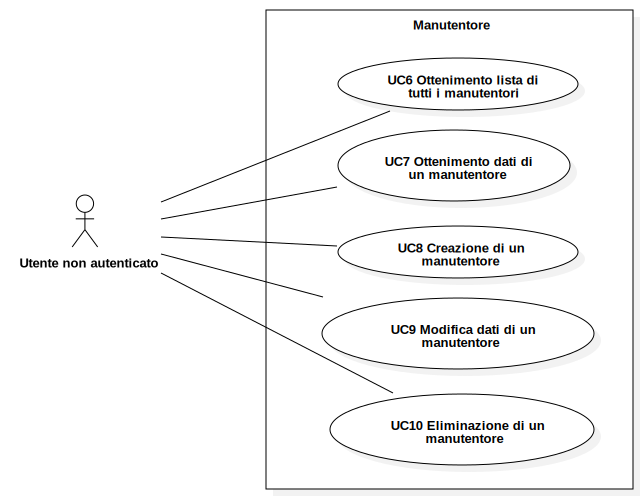
\includegraphics[height=9cm]{usecase/maintainer}
\end{figure}
\textbf{UC6 - Ottenimento lista di tutti i manutentori}
\\\\
\textbf{Attori primari:} utente non autenticato.
\\
\textbf{Precondizioni:} l'utente è in possesso degli strumenti per poter effettuare la richiesta al sistema.
\\
\textbf{Post-condizioni:} l'utente ha ottenuto una lista di tutti i manutentori.
\\
\textbf{Scenario principale:}
\begin{enumerate}
    \item l'utente richiede la lista di tutti i manutentori.
    \item l'utente ottiene una lista di tutti i manutentori.
\end{enumerate}
\leavevmode\newline
\textbf{UC7 - Ottenimento dati di un manutentore}
\\\\
\textbf{Attori primari:} utente non autenticato.
\\
\textbf{Precondizioni:} l'utente è in possesso degli strumenti per poter effettuare la richiesta al sistema.
\\
\textbf{Post-condizioni:} l'utente ha ottenuto i dati di un manutentore.
\\
\textbf{Scenario principale:}
\begin{enumerate}
    \item l'utente richiede i dati di un manutentore.
    \item l'utente ottiene i dati di un manutentore.
\end{enumerate}
\leavevmode\newline
\textbf{UC8 - Creazione di un manutentore}
\\\\
\textbf{Attori primari:} utente non autenticato.
\\
\textbf{Precondizioni:} l'utente è in possesso degli strumenti per poter effettuare la richiesta al sistema.
\\
\textbf{Post-condizioni:} l'utente ha creato un manutentore.
\\
\textbf{Scenario principale:}
\begin{enumerate}
    \item l'utente richiede la creazione di un manutentore.
    \item l'utente crea un manutentore.
\end{enumerate}
\leavevmode\newline
\textbf{UC9 - Modifica dati di un manutentore}
\\\\
\textbf{Attori primari:} utente non autenticato.
\\
\textbf{Precondizioni:} l'utente è in possesso degli strumenti per poter effettuare la richiesta al sistema.
\\
\textbf{Post-condizioni:} l'utente ha modificato un manutentore.
\\
\textbf{Scenario principale:}
\begin{enumerate}
    \item l'utente richiede la modifica di un manutentore.
    \item l'utente modifica un manutentore.
\end{enumerate}
\leavevmode\newline
\textbf{UC10 - Eliminazione di un manutentore}
\\\\
\textbf{Attori primari:} utente non autenticato.
\\
\textbf{Precondizioni:} l'utente è in possesso degli strumenti per poter effettuare la richiesta al sistema.
\\
\textbf{Post-condizioni:} l'utente ha eliminato un manutentore.
\\
\textbf{Scenario principale:}
\begin{enumerate}
    \item l'utente richiede l'eliminazione di un manutentore.
    \item l'utente elimina un manutentore.
\end{enumerate}

% sensore
\leavevmode\newline
\begin{figure}[!h]
    \centering
    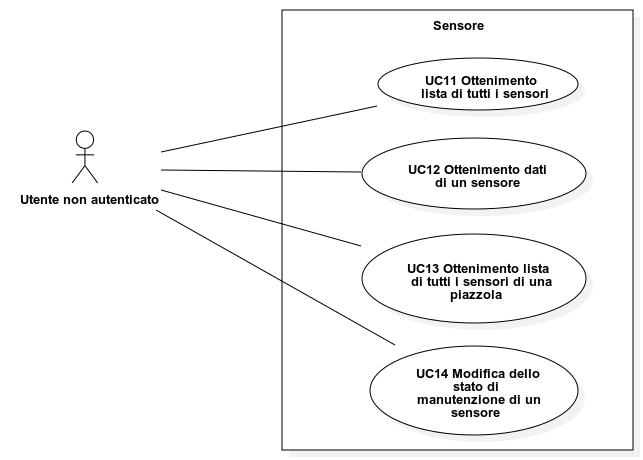
\includegraphics[height=9cm]{usecase/sensor}
\end{figure}
\textbf{UC11 - Ottenimento lista di tutti i sensori}
\\\\
\textbf{Attori primari:} utente non autenticato.
\\
\textbf{Precondizioni:} l'utente è in possesso degli strumenti per poter effettuare la richiesta al sistema.
\\
\textbf{Post-condizioni:} l'utente ha ottenuto una lista di tutti i sensori.
\\
\textbf{Scenario principale:}
\begin{enumerate}
    \item l'utente richiede la lista di tutti i sensori.
    \item l'utente ottiene una lista di tutti i sensori.
\end{enumerate}
\leavevmode\newline
\textbf{UC12 - Ottenimento dati di un sensore}
\\\\
\textbf{Attori primari} utente non autenticato.
\\
\textbf{Precondizioni:} l'utente è in possesso degli strumenti per poter effettuare la richiesta al sistema.
\\
\textbf{Post-condizioni:} l'utente ha ottenuto i dati di un sensore.
\\
\textbf{Scenario principale:}
\begin{enumerate}
    \item l'utente richiede i dati di un sensore.
    \item l'utente ottiene i dati di un sensore.
\end{enumerate}
\leavevmode\newline
\textbf{UC13 - Ottenimento lista di tutti i sensori di una piazzola}
\\\\
\textbf{Attori primari:} utente non autenticato.
\\
\textbf{Precondizioni:} l'utente è in possesso degli strumenti per poter effettuare la richiesta al sistema.
\\
\textbf{Post-condizioni:} l'utente ha ottenuto una lista di tutti i sensori di una piazzola.
\\
\textbf{Scenario principale:}
\begin{enumerate}
    \item l'utente richiede la lista di tutti i sensori di una piazzola.
    \item l'utente ottiene una lista di tutti i sensori di una piazzola.
\end{enumerate}
\leavevmode\newline
\textbf{UC14 - Modifica dello stato di manutenzione di un sensore}
\\\\
\textbf{Attori primari:} utente non autenticato.
\\
\textbf{Precondizioni:} l'utente è in possesso degli strumenti per poter effettuare la richiesta al sistema.
\\
\textbf{Post-condizioni:} l'utente ha modificato lo stato di manutenzione di un sensore.
\\
\textbf{Scenario principale:}
\begin{enumerate}
    \item l'utente richiede la modifica dello stato di manutenzione di un sensore.
    \item l'utente modifica lo stato di manutenzione di un sensore.
\end{enumerate}

% piazzola
\leavevmode\newline
\begin{figure}[!h]
    \centering
    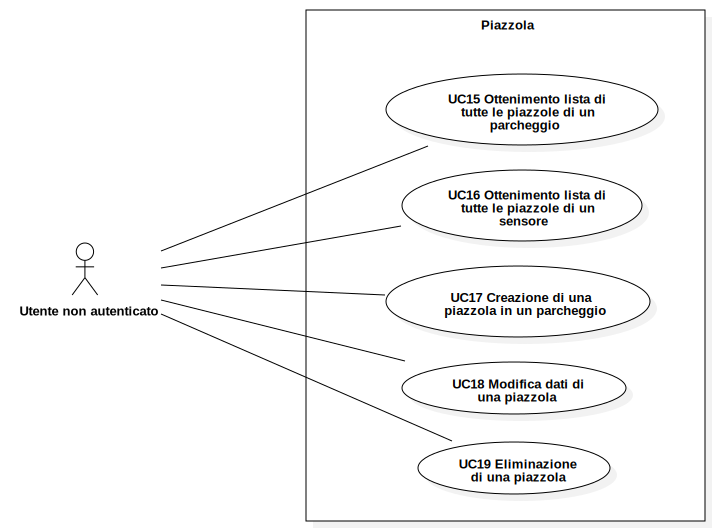
\includegraphics[height=9cm]{usecase/parking-spot}
\end{figure}
\textbf{UC15 - Ottenimento lista di tutte le piazzole di un parcheggio}
\\\\
\textbf{Attori primari:} utente non autenticato.
\\
\textbf{Precondizioni:} l'utente è in possesso degli strumenti per poter effettuare la richiesta al sistema.
\\
\textbf{Post-condizioni:} l'utente ha ottenuto una lista di tutte le piazzole di un parcheggio.
\\
\textbf{Scenario principale:}
\begin{enumerate}
    \item l'utente richiede la lista di tutte le piazzole di un parcheggio.
    \item l'utente ottiene una lista di tutte le piazzole di un parcheggio.
\end{enumerate}
\leavevmode\newline
\textbf{UC16 - Ottenimento lista di tutte le piazzole di un sensore}
\\\\
\textbf{Attori primari:} utente non autenticato.
\\
\textbf{Precondizioni:} l'utente è in possesso degli strumenti per poter effettuare la richiesta al sistema.
\\
\textbf{Post-condizioni:} l'utente ha ottenuto una lista di tutte le piazzole di un sensore.
\\
\textbf{Scenario principale:}
\begin{enumerate}
    \item l'utente richiede la lista di tutte le piazzole di un sensore.
    \item l'utente ottiene una lista di tutte le piazzole di un sensore.
\end{enumerate}
\leavevmode\newline
\textbf{UC17 - Creazione di una piazzola in un parcheggio}
\\\\
\textbf{Attori primari:} utente non autenticato.
\\
\textbf{Precondizioni:} l'utente è in possesso degli strumenti per poter effettuare la richiesta al sistema.
\\
\textbf{Post-condizioni:} l'utente ha creato una piazzola in un parcheggio.
\\
\textbf{Scenario principale:}
\begin{enumerate}
    \item l'utente richiede la creazione di una piazzola in un parcheggio.
    \item l'utente crea una piazzola in un parcheggio.
\end{enumerate}
\leavevmode\newline
\textbf{UC18 - Modifica dati di una piazzola}
\\\\
\textbf{Attori primari:} utente non autenticato.
\\
\textbf{Precondizioni:} l'utente è in possesso degli strumenti per poter effettuare la richiesta al sistema.
\\
\textbf{Post-condizioni:} l'utente ha modificato una piazzola.
\\
\textbf{Scenario principale:}
\begin{enumerate}
    \item l'utente richiede la modifica di una piazzola.
    \item l'utente modifica una piazzola.
\end{enumerate}
\leavevmode\newline
\textbf{UC19 - Eliminazione di una piazzola}
\\\\
\textbf{Attori primari:} utente non autenticato.
\\
\textbf{Precondizioni:} l'utente è in possesso degli strumenti per poter effettuare la richiesta al sistema.
\\
\textbf{Post-condizioni:} l'utente ha eliminato una piazzola.
\\
\textbf{Scenario principale:}
\begin{enumerate}
    \item l'utente richiede l'eliminazione di una piazzola.
    \item l'utente elimina una piazzola.
\end{enumerate}

% misurazione
\leavevmode\newline
\begin{figure}[!h]
    \centering
    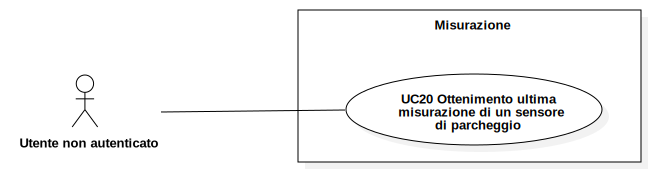
\includegraphics[height=9cm]{usecase/parking-sensor}
\end{figure}
\textbf{UC20 - Ottenimento ultima misurazione di un sensore di parcheggio}
\\\\
\textbf{Attori primari:} utente non autenticato.
\\
\textbf{Precondizioni:} l'utente è in possesso degli strumenti per poter effettuare la richiesta al sistema.
\\
\textbf{Post-condizioni:} l'utente ha ottenuto l'ultima misurazione di un sensore di parcheggio.
\\
\textbf{Scenario principale:}
\begin{enumerate}
    \item l'utente richiede l'ultima misurazione di un sensore di parcheggio.
    \item l'utente ottiene l'ultima misurazione di un sensore di parcheggio.
\end{enumerate}

% polling sensore
\leavevmode\newline
\textbf{UC21 - Ottenimento lista di tutte le piazzole di un parcheggio}
\\\\
\textbf{Attori primari:} utente non autenticato.
\\
\textbf{Precondizioni:} l'utente è in possesso degli strumenti per poter effettuare la richiesta al sistema.
\\
\textbf{Post-condizioni:} l'utente ha ottenuto una lista di tutte le piazzole di un parcheggio.
\\
\textbf{Scenario principale:}
\begin{enumerate}
    \item l'utente richiede la lista di tutte le piazzole di un parcheggio.
    \item l'utente ottiene una lista di tutte le piazzole di un parcheggio.
\end{enumerate}

% //TODO: inserire sotto casi d'uso specificando i campi da visualizzare / modificare
\section{Tracciamento dei requisiti}
Ogni requisito è identificato da un codice univoco nel seguente formato:
\begin{itemize}
    \item la prima lettera è sempre R, a indicare la parola requisito
    \item la seconda lettera indica il tipo di requisito:
    \begin{itemize}
        \item F per i requisiti funzionali
        \item Q per i requisiti qualitativi
        \item V per i requisiti di vincolo
    \end{itemize}
    \item un numero progressivo che identifica in modo univoco il requisito.
\end{itemize}
Per maggior chiarezza i requisiti sono stati raggruppati per entità di dominio di appartenenza.
% //TODO: inserire casi d'uso sensors-scraping
% //TODO: inserire requisiti funzionali sensors-scraping
% parcheggio
\leavevmode\newline
\begin{table}
    \begin{tabular}{|p{1cm}|p{6cm}|p{1.9cm}|p{1.8cm}|} 
    \hline
    Codice & Descrizione & Rilevanza &  Fonti \\ 
    \hline
    RF1 & L'utente non autenticato deve poter ottenere la lista di tutti i parcheggi. & Obbligatorio & UC1 \\ 
    \hline
    RF2 & L'utente non autenticato deve poter ottenere i dati di un parcheggio. & Obbligatorio & UC2 \\ 
    \hline
    RF3 & L'utente non autenticato deve poter creare un parcheggio. & Obbligatorio & UC3 \\ 
    \hline
    RF4 & L'utente non autenticato deve poter modificare i dati di un parcheggio. & Obbligatorio & UC4 \\
    \hline
    RF5 & L'utente non autenticato deve poter eliminare un parcheggio. & Obbligatorio & UC5 \\ 
    \hline
    \end{tabular}
\end{table}

% manutentore
\leavevmode\newline
\begin{table}
    \begin{tabular}{|p{1cm}|p{6cm}|p{1.9cm}|p{1.8cm}|} 
    \hline
    Codice & Descrizione & Rilevanza &  Fonti \\ 
    \hline
    RF6 & L'utente non autenticato deve poter ottenere la lista di tutti i manutentori. & Obbligatorio & UC6 \\ 
    \hline
    RF7 & L'utente non autenticato deve poter ottenere i dati di un manutentore. & Obbligatorio & UC7 \\ 
    \hline
    RF8 & L'utente non autenticato deve poter creare un manutentore. & Obbligatorio & UC8 \\ 
    \hline
    RF9 & L'utente non autenticato deve poter modificare i dati di un manutentore. & Obbligatorio & UC9 \\
    \hline
    RF10 & L'utente non autenticato deve poter eliminare un manutentore. & Obbligatorio & UC10 \\ 
    \hline
    \end{tabular}
\end{table}

% sensore
\leavevmode\newline
\begin{table}
    \begin{tabular}{|p{1cm}|p{6cm}|p{1.9cm}|p{1.8cm}|} 
    \hline
    Codice & Descrizione & Rilevanza &  Fonti \\ 
    \hline
    RF11 & L'utente non autenticato deve poter ottenere la lista di tutti i sensori. & Obbligatorio & UC11 \\ 
    \hline
    RF12 & L'utente non autenticato deve poter ottenere i dati di un sensori. & Obbligatorio & UC12 \\ 
    \hline
    RF13 & L'utente non autenticato deve poter ottenere la lista di tutti i sensori di una piazzola. & Obbligatorio & UC13 \\ 
    \hline
    RF14 & L'utente non autenticato deve poter modificare lo stato di manutenzione di un sensore. & Obbligatorio & UC14 \\ 
    \hline
    \end{tabular}
\end{table}

% piazzola
\leavevmode\newline
\begin{table}
    \begin{tabular}{|p{1cm}|p{6cm}|p{1.9cm}|p{1.8cm}|} 
    \hline
    Codice & Descrizione & Rilevanza &  Fonti \\ 
    \hline
    RF15 & L'utente non autenticato deve poter ottenere la lista di tutte le piazzole di un parcheggio. & Obbligatorio & UC15 \\ 
    \hline
    RF16 & L'utente non autenticato deve poter ottenere la lista di tutte le piazzole di un sensore. & Obbligatorio & UC16 \\ 
    \hline
    RF17 & L'utente non autenticato deve poter creare una piazzola in un parcheggio. & Obbligatorio & UC17 \\ 
    \hline
    RF18 & L'utente non autenticato deve poter modificare i dati di una piazzola. & Obbligatorio & UC18 \\
    \hline
    RF19 & L'utente non autenticato deve poter eliminare una piazzola. & Obbligatorio & UC19 \\
    \hline
    \end{tabular}
\end{table}

% misurazione
\leavevmode\newline
\begin{table}
    \begin{tabular}{|p{1cm}|p{6cm}|p{1.9cm}|p{1.8cm}|} 
    \hline
    Codice & Descrizione & Rilevanza &  Fonti \\ 
    \hline
    RF20 & L'utente non autenticato deve poter ottenere l'ultima misurazione di un sensore di parcheggio. & Obbligatorio & UC20 \\ 
    \hline
    \end{tabular}
\end{table}

% requisiti di qualità
\leavevmode\newline
\begin{table}
    \begin{tabular}{|p{1cm}|p{6cm}|p{1.9cm}|p{1.8cm}|} 
    \hline
    Codice & Descrizione & Rilevanza &  Fonti \\ 
    \hline
    RQ1 & Deve essere presente una suite di test automatici per testare la business logic con una copertura a livello branch
        >= 90\%. & Obbligatorio & Capitolato \\ 
    \hline
    RQ2 & Deve essere presente una suite di test automatici per testare la business logic con una copertura a livello linee
        di codice >= 60\%. & Obbligatorio & Capitolato \\ 
    \hline
    RQ3 & Deve essere presente una documentazione che spieghi le scelte progettuali fatte e i motivi che hanno portato ad effettuare
        tali scelte. & Obbligatorio & Capitolato \\ 
    \hline
    \end{tabular}
\end{table}

% requisiti di vincolo
\leavevmode\newline
\begin{table}
    \begin{tabular}{|p{1cm}|p{6cm}|p{1.9cm}|p{1.8cm}|} 
    \hline
    Codice & Descrizione & Rilevanza &  Fonti \\ 
    \hline
    RV1 & Utilizzo del framework NestJS per realizzare l'applicazione. & Obbligatorio & Capitolato \\ 
    \hline
    RV2 & Utilizzo di database PostgreSQL. & Desiderabile & Capitolato \\ 
    \hline
    RV3 & Le REST API devono poter essere chiamate tramite protocollo HTTP. & Obbligatorio & Capitolato \\ 
    \hline
    RV4 & La richiesta di ottenimento delle entità, all'applicazione, deve essere fatta tramite metodo GET. & 
        Obbligatorio & Capitolato \\ 
    \hline
    RV5 & La richiesta di inserimento delle entità, all'applicazione, deve essere fatta tramite metodo POST. & 
        Obbligatorio & Capitolato \\ 
    \hline
    RV6 & La richiesta di modifica delle entità, all'applicazione, deve essere fatta tramite metodo PUT. & 
        Obbligatorio & Capitolato \\ 
    \hline
    RV7 & La richiesta di cancellazione delle entità, all'applicazione, deve essere fatta tramite metodo DELETE. & 
        Obbligatorio & Capitolato \\ 
    \hline
    \end{tabular}
\end{table}